\documentclass{article}
\usepackage{graphicx} % Required for inserting images
\usepackage{fullpage}
\usepackage{url}
\usepackage{hyperref} 
\usepackage{pgfplots}
\pgfplotsset{compat=1.18}
\usepackage{pgfplotstable}
\usepackage{multicol}

\usepackage{subcaption}
\usepackage{algorithm}
\usepackage{float}
\usepackage{algpseudocode}
\usepackage{amsmath}

\usepackage{titlesec}
\titlespacing\section{0pt}{12pt plus 4pt minus 2pt}{8pt plus 2pt minus 2pt}
\titlespacing\subsection{0pt}{11pt plus 4pt minus 2pt}{6pt plus 2pt minus 2pt}

\graphicspath{ {./imgs/}  }

\title{FROGBYTE HPC F25}
\author{ANNA NORRIS\\CARMEN PARK\\DAVID HADDAD\\STELLA GREENVOSS}
\date{\today}


\begin{document}

\maketitle


\begin{center}
WITH JEE CHOI\\[100pt]
\end{center}

\begin{abstract}
This paper evaluates sparse matrix-vector multiplication (SpMV) performance across five storage formats: CSR, COO, ELL, SELL-C, and CSR5. We discuss each kernel and corresponding storage format, as well as their performance with respect to matrix size and sparsity patterns. We then implement each format with architecture-specific optimizations; benchmarking across matrices with varying sparsity patterns. We discuss how we developed our interpretations of each implementation, and what improvements could be made in the future. Our results indicate trade-offs between memory efficiency and computational throughput that inform format selection for target hardware, and help inform when each kernel is the most effective. We additionally propose further work that can be done to further evaluate and improve these kernels.\\[60pt]
\end{abstract}


\begin{multicols}{2}
\section{Introduction}

Sparse Matrix-Vector (SpMV) multiplication is a fundamental operation in scientific computing and graph analytics. It efficiently computes the product $y = Ax$ of a sparse matrix $A$ and a vector $x$ by performing operations only on the nonzero elements. This significantly reduces the computational cost compared to carrying out useless computations on zeroes. Optimizing SpMV is also multifaceted in that there are numerous SPMV computational kernels – many of which use their own unique storage formats – and routines within larger processes that each have their own parallelization requirements.  \newline


Through the course of this project, the FrogByte team conducted a comprehensive examination of both naive and parallel implementations of standard sparse matrix-vector multiplication (SpMV) formats, including ELLPACK (ELL), Coordinate (COO), and Compressed Sparse Row (CSR). Beyond these more conventional storage formats, we further investigated and implemented advanced hybrid formats such as the Sliced ELLPACK-C-$\sigma$ (SELL-C-$\sigma$) and CSR5 formats, which are both designed to address specific performance bottlenecks on modern GPU architectures. Finally, we began to investigate and profile Vector-COO/CSR. Our research aimed to systematically compare the performance characteristics of each format's kernel implementation across a diverse range of matrix sparsity patterns, including regular, irregular, and highly irregular nonzero distributions, as well as matrices exhibiting both uniform and skewed density profiles. 

All benchmarking and comparative analysis were executed on high-performance computing platforms; specifically, the University of Oregon’s Talapas cluster and Portland State University's ORCA system, with particular emphasis on evaluating scalability and architectural efficiency across different parallel implementations.

\section{Background and Related Work}
SpMV is a crucial operation in scientific computing. It can be utilized in many scientific and mathematical disciplines, ranging between linear solvers, eigenvalue problems, graph algorithms, and more. One computational characteristic of SpMV is that it is memory-bound. This often means that irregular memory access patterns cause a significant bottleneck for computation, lowering the overall execution time. Matrix size is thus a significant slowdown factor in these operations. The SpMV problem formulation is $y = A·x$ where $A$ is an $m*n$ sparse matrix and $x$ is a size $n$ vector. 

\subsection{Traditional SpMV Storage Formats}
Traditional sparse matrix storage formats each present distinct trade-offs between structural regularity and flexibility. The Coordinate (COO) format offers maximal flexibility through simple triple storage (row, column, value) but suffers from poor cache locality and inefficient memory access patterns. In contrast, the Compressed Sparse Row (CSR) format — the CPU standard — organizes data by row for better spatial locality but introduces load imbalance challenges on parallel architectures. The ELLPACK (ELL) format enforces structural regularity through uniform row padding to enable coalesced GPU memory access, achieving high performance for uniform matrices but incurring prohibitive padding overhead for irregular patterns.
\subsubsection{COO}
The Coordinate (COO) format represents the most intuitive sparse matrix storage scheme. It encodes the non-zero numbers, column indices, and row indices in three separate arrays, so there are three arrays of size equal to the number of non-zeros.
\subsubsection{CSR}
The Compressed Sparse Row (CSR) format has emerged as the de-facto standard for sparse matrix storage in CPU-based scientific computing, organizing non-zero numbers into three arrays: row pointers indicating the start of each row, column indices for each nonzero, and corresponding values. This row-major organization provides efficient sequential access to all elements within a row, making it particularly suitable for iterative solvers and algorithms with row-wise dependencies. 
\subsubsection{ELL}
The ELLPACK (ELL) format addresses GPU memory coalescing requirements by enforcing a regular structure through uniform row padding. In ELL representation, all rows are padded to equal length with data stored in two dense 2D arrays: one for column indices and another for values. This regularity enables perfectly coalesced memory accesses when threads within a warp process corresponding elements across different rows, maximizing memory bandwidth utilization on GPU architectures. However, the row length is determined by calculating the maximum number of nonzero entries in a row in a matrix. Thus, a matrix with a low average number of nonzero entries per row with a significant dense row outlier will waste space and time spent allocating padded rows. 

\section{GPU Considerations}

With the rise of GPU computing, the need for faster SpMV operations has become increasingly critical. This has led to the modification and altering of traditional SpMV formats to better address factors like
\begin{itemize}
\item Memory Coalescing, 
\item Warp Divergence, 
\item Occupancy Limitations, 
\item Latency Hiding, and
\item Memory Hierarchy.
\end{itemize}


Uncoalesced memory accesses often degrade bandwidth utilization, and thread under-utilization during memory latency stalls. These limitations have catalyzed research into GPU-optimized sparse formats that impose structural regularity not unlike ELL's uniform padding, or use sophisticated load balancing strategies. This is reshaping how many sparse matrices are stored and processed to better align with GPU execution characteristics.  What SELL-C-$\sigma$ and CSR5 focus on is building upon existing formats, ELL and CSR respectively, and more evenly distributing the work load within the GPU architecture as well as localizing where the work is done so it can be more efficiently computed by each thread block or SIMD lane and fully saturate the GPU's compute units.

This can similarly be seen with the COO and CSR warp level approach, seen in Tsai et al. \cite{Tsai2021Race} where each warp processes one or more rows of the sparse matrix. This level of optimization has become a new standard to seek out with parallelized sparse vector matrix operations, and the root of our current exploration.


\section{Advanced SpMV for GPUs}
\subsection{SELL-C-$\sigma$}

Among the many optimized GPU formats in recent literature, the Sliced ELLPACK-C-$\sigma$ (SELL-C-$\sigma$) format demonstrates and exploits the clear trade-offs made by many naive formats (specifically CSR and ELL). A pseudo-hybrid model, SELL-C-$\sigma$, extends ELL by dividing the matrix into fixed-height slices of size $C$ rows and applying row reordering locally to each slice. This reordering is dependent on $\sigma$ and attempts to decrease the amount of padding overhead seen in the ELL method on irregular matrices.

ELL solves the memory coalescing problem introduced on the GPU when running CSR. This reordering of data and the benefit we see is even greater for SELL-C-$\sigma$. All threads within a warp load memory coalesced. This allowed the SELL-C-$\sigma$ kernel to perform well across all our initial testing, often outperforming CSR and ELL.

\subsubsection{SELL-C-$\sigma$ Storage Format and Conversion}

The SELL-C-$\sigma$ format improves on ELL by slicing the matrix into blocks of $C$ consecutive rows (pre-sort). The parameter $C$ is chosen to match the size of the warp (in our case $C=32$). Inside each slice, the rows are sorted by length (nonzero count), and in our implementation, this is maintained locally to avoid disturbing the global row order ($\sigma=C$). 

Padding is determined locally within each slice, based on the same ELL metric of the maximum row length. The effect is a drastic reduction in padding overhead compared to a naive ELL implementation, while maintaining the uniform coalesced memory access. The slices are stored in two arrays, one for column indices and one for values. Column-major ordering of these allows for threads to perform fully coalesced memory access throughout the processing of a row.

The CPU-side conversion also introduces overhead, but it is negligible after a certain number of SpMV operations (depending on the matrix size), so it is amortized in the typical use case where hundreds of operations take place on the GPU before transferring back to the host. The CPU performs slicing, nonzero counting in each slice, sorting, and matrix padding. An array for mapping row sorting is recorded to allow recovery of the original matrix row ordering after GPU computation, if needed.

\subsubsection{SELL-C-$\sigma$ Kernel}
The SELL-C-$\sigma$ kernel launches a warp per row-slice (larger workload than per row). Since $C$ is set to the size of the warp, each thread within the warp is assigned to a specific row within the slice. All the rows are the same length, allowing identical loop bounds and eliminating branch divergence on the GPU. As stated before, this allows memory transactions to be coalesced.

The execution of the kernel involves iterating over the padded slice, loading a column index and value each iteration. The vector entry corresponding to the column is read, multiplied, and accumulated. Theoretically, the kernel maximizes memory throughput with this structure, as all threads have identical memory access patterns. After the slice has computed its values, the threads write their accumulated values to the output vector (reducing the number of atomic operations). The CPU then unscrambles the row ordering.

\subsection{CSR5}

CSR5 (Compressed Sparse Row version 5) is a tile-based sparse matrix format introduced by Liu and Vinter in 2015 \cite{Liu2015CSR5} designed explicitly for efficient SpMV operations across diverse parallel architectures, including both CPUs and GPUs. Unlike traditional formats that optimize for either regularity or flexibility, CSR5 employs a balanced approach that partitions the matrix into uniform tiles while maintaining the computational simplicity of CSR through auxiliary data structures for load balancing. It transposes traditional CSR value and column arrays into $s\omega x \sigma$ sized tiles to help with contiguous memory access and to break up work into warp level chunks. There are a few additional elements that are added as a result to also speed up processing.


\subsubsection{CSR5 Storage Format}

The CSR5 format organizes sparse matrices through several key data structures that enable both efficient storage and parallel computation. For example, the tile size ($\sigma \times \omega$) is hardware dependent, where  $\omega$ (tile width) is primarily determined by hardware characteristics such as warp size, while $\sigma$ (tile height) depends on both hardware constraints and the sparsity pattern of the matrix.

To clearly process each tile, two additional peices of information, a tile pointer, and a tile descriptor, are created to speed up tile processing. The tile pointer, which is the length of the total numbers of tiles, indicates the row number of the first element in each tile.

The tile descriptor is composed of 4 parts: \texttt{bit\_flag}, \texttt{y\_offset}, \texttt{seg\_offset}, and \texttt{empty\_offset}. Each plays a key role in assuring accurate results and optimizing parallelization.

\begin{itemize}
\item \texttt{bit\_flag}: The \texttt{bit\_flag} is an indicator of the start of a new row. This covers the size of \texttt{num\_tiles} $\times \omega \times \sigma$ but often with at least half the space of double precision floats. We experimented with storing \texttt{bit\_flag} in \texttt{uint32\_t} as well as \texttt{uint8\_t} tiles.

\item \texttt{y\_offset}: The \texttt{y\_offset} can be obtained by counting the number of true flags in the columns preceding it. This array is size $\omega$ for every tile, and is helpful in indicating where partial sums can best be stored.

\item \texttt{seg\_offset}:  The segmentation offset, which is also size $\omega$ for each tile, indicates how many tile columns to its right are within the same row in the sparse matrix. The purpose of this allows the kernel to take each tile column and break its product into a set of prefix sum operations. These partial sums across each tile contribute to further optimizations in performance.   

\item \texttt{empty\_offset}: The \texttt{empty\_offset} array is the length of the number of rows in a tile, and is only needed if there exists an empty row in the tile. This array is usually the smallest of the descriptors, but crucial for accurate results on CSR5.

\end{itemize}


The CSR5 SpMV kernel employs a two-phase execution strategy optimized for parallel architectures:
\textbf{Phase 1: Tile Processing}
\begin{itemize}
\item Each thread block or SIMD lane processes one or more complete tiles
\item Threads within a warp cooperate on tile computation using warp-level primitives
\item The bit-flag array directs threads to valid elements, avoiding computation on padding
\item Partial results are accumulated using efficient warp-level reduction operations
\end{itemize}
\textbf{Phase 2: Row Accumulation}
\begin{itemize}
\item Partial results from tiles contributing to the same output row are combined
\item Atomic operations or segmented reduction techniques merge contributions
\item Row versioning information ensures correct mapping to output vector y
\end{itemize}
\textbf{Key Optimizations:}
\begin{enumerate}
\item \textbf{Warp-Centric Execution}: Each warp processes entire tiles, maintaining SIMD efficiency
\item \textbf{Bit-Level Masking}: The bit-flag array acts as a map to help detect when 
\item \textbf{Memory Coalescing}: Tile organization ensures contiguous memory access patterns
\item \textbf{Load Balancing}: The $\sigma$ parameter controls tile grouping to balance workloads across warps
\end{enumerate}


\section{methodology}


Our computational approach employs multiple sparse matrix storage formats to analyze their suitability for specific algorithmic patterns. In the following section we discuss the implementation of the five key representations from above, CSR, COO , ELL, SELL-C, and CSR5. This evaluation is conducted through systematic benchmarking on diverse sparse matrices, measuring both memory footprint and computational throughput.


To ensure correctness across different architectures, these kernels were profiled on two different HPC clusters: Talapas, the University of Oregon’s cluster, and ORCA, PSU’s cluster. On Talapas, we used a single NVIDIA A100 GPU (Ampere architecture) with 40 GB HBM2 memory, 1.6 TB/s memory bandwidth, and 9.7 TFLOPS double-precision peak performance.
 On ORCA, we used an L40S, which uses NVIDIA Ada Lovelace Architecture, has 40GB GDDR6 memory, and 864 GB/s memory bandwidth. For each metric and comparison, we specify which cluster it was collected on. We did not include multi-node functionality in order to control the scope of our project. 


\subsection{COO}

There are a number of ways to implement COO SpMV in GPU programming. In this instance, we attempted to implement three versions: scalar COO, vector COO, and another more complex load-balancing vector COO. In the case of scalar COO programmed in CUDA, it resembles the sequential version the most. In this case, a thread is assigned to an index of the arrays and performs atomic addition to add the product to the result vector. We find the number of blocks by dividing the size of the rows by the number of threads in a block.  This implementation has a number of obvious drawbacks, including poor memory locality and the frequent use of atomic addition leads to significant performance overhead. \newline

The vector COO kernel we implemented assigns one warp of 32 threads to a chunk of COO entries. Then, it iterates in a grid-stride loop and after loading data, performs warp-level reduction to find the partial-sum of the warp. Then, the last thread in the segment uses \texttt{atomicAdd} to add the value to the result vector. This kernel improves on the format of the scalar COO kernel by reducing the number of \texttt{atomicAdd} from one per COO entry to one per warp. However, the issue of poor memory locality remains, and this version of vector COO SpMV results in a load imbalance between warps so performance is worsened.\newline

We were unable to achieve accurate results with our implementation of a third load-balancing COO kernel, this will be revisited in future work. We followed the algorithm given in the Tsai Y., et al. paper \cite{Tsai2021Race}. One significant detail for this kernel is that it expects sorted COO arrays by row then column. This is because it assumes the arrays are sorted to compute whether the warp will encounter the next row. If it does, then it performs a segmented scan to collect the partial-sum of the current row, and the first thread of the segment performs the atomic addition. One deviation in our implementation is that the last thread in the segment performs the atomic addition and adjusted the segmented scan accordingly, but again, due to inaccurate results with our implementation it was not included when measuring performance.

\begin{algorithm}[H]
\caption{Load-balancing COO kernel algorithm}
\label{alg:lb-coo}
\begin{algorithmic}[1]
\State ind $\gets$ index of the first element to be processed by this thread
\State current\_row $\gets$ \texttt{rowidx[ind]}
\State $c \gets A[\texttt{ind}] \times x[\texttt{colidx[ind}]]$
\For{$i = 0$ \textbf{to} \texttt{nz\_per\_warp} \textbf{step} \texttt{warpsize}}
    \State next\_row $\gets$ \texttt{rowidx[next ind]}
    \If{\textbf{any thread} has next\_row $\neq$ current\_row \textbf{ or final iteration}}
        \State Perform segmented scan for the current row
        \If{this thread is first in its segment}
            \State \texttt{atomicAdd}(output[current\_row], $c$)
        \EndIf
        \State $c \gets 0$
    \EndIf
    \State ind $\gets$ \texttt{next ind}
    \State $c \gets c + A[\texttt{ind}] \times x[\texttt{colidx[ind}]]$
    \State current\_row $\gets$ next\_row
\EndFor
\end{algorithmic}
\end{algorithm}


\subsection{CSR}

Similarly to COO, we implemented scalar and vector versions of CSR SpMV. Once again, the scalar version is the easiest to implement because of its similarities to the serial version of CSR. In this case, one thread is assigned to one row in the CSR array and the sum of the product of all values in the row are added to the result vector by the thread. We divide the number of rows by the number of threads per block to find the number of blocks needed. This version has poor memory coalescence because threads will access non-contiguous entries and can have significant load-imbalance with irregular matrices.\newline

In order to improve on scalar CSR, we created a vector CSR kernel as well. In this case, a warp of 32 threads is assigned to a single row in the matrix and this computes the product of that row. Then, warp reduction is performed to create the sum that is written to the output vector. This version will more effectively utilize memory locality because the threads in the warp are sequentially accessing the same segments of memory. The following pseudo code as provided in the Tsai Y., et al. paper is what we used for our implementation.\newline

\begin{algorithm}[H]
\caption{Vector CSR kernel}
\label{alg:ginkgo-csr}
\begin{algorithmic}[1]
\State row $\gets$ \text{row index for this thread}
\State subrow $\gets$ \text{stride to next row}
\State step\_size $\gets$ \text{stride to next element}
\State $c \gets 0$
\For{$\text{row} = \text{row}$ \textbf{to} \#rows \textbf{step} subrow}
    \For{$\text{idx} = \texttt{rowptr[row]}$ \textbf{to} \texttt{rowptr[row+1]} \textbf{step} step\_size}
    \State $c \gets c + \texttt{val[idx]} \times b[\texttt{col[idx]}]$
    \EndFor
    \State Perform warp reduction on $c$
    \If{thread 0 in subwarp}
        \State Write $c$ to output[row]
    \EndIf
\EndFor
\end{algorithmic}
\end{algorithm}
\subsection{CSR5}

We utilized the already constructed CSR arrays to create CSR5 for this project. The git repository connected to Liu's original work \cite{Liu2015CSR5} seemed to pull CSR5 directly from a matrix file which could be an interesting attempt in the future.

To determine the optimal $\sigma$ bounds ⟨r, s, t, u⟩ for a given GPU, you can perform hardware benchmarks using a set of fabricated sparse matrices with controlled uniform row densities. The process will show CSR5 SpMV performance across a wide range of $\sigma$ values for each matrix density. You identify r as the point where too-small of a $\sigma$ degrades performance for sparse rows. Similarly, s is the optimal $\sigma$ for moderate densities; and $t$ becomes the threshold where a larger $\sigma$ value no longer is beneficial. U becomes the most optimal and often small $\sigma$ for extremely dense rows. These hardware-dependent values are fixed once established through this initialization benchmark, and there is no need for parameter tuning for all subsequent SpMV executions. 

In implementing CSR5, creating the tile pointer was relatively straightforward, while there were a lot of spaces for interpretation of how to gather together the tile descriptor. As far as memory allocation, writing the value and column arrays to 2D tiles led to the use of \texttt{CudaMallocPitch} for tiling, and copying the row pointer was similar to homework 3 and 4 in that the memory from the CPU was copied to global GPU memory. 

First implementations of gathering the tile descriptor and the tile pointer took place serially on the CPU. For the tile pointer this meant incrementing through the tiles and finding the initial row index.

For the tile descriptor, naive attempts also stayed on serial on the CPU. This involved using the row pointer to write a comprehensive \texttt{bit\_flag} array, then using its dimensions to build each tiles $\texttt{y\_offset}$ array and $\texttt{seg\_offset}$ array. Constructing the \texttt{empty\_array} proved to be the most difficult. It was also initially allocated in C++, but each array's length varied based off of the number of rows in the empty tile. 

There is pseudo code in Liu et al \cite{Liu2015CSR5} that finds tile descriptor elements on the GPU. Looking more closely at this implementation could be promising for a faster and more efficient collection of each descriptor variable.  


\subsection{ELL}

The ELLPACK (ELL) format restructures the sparse matrix into two dense 
$\text{\texttt{num\_rows}} \times L$ arrays, where $L$ is the maximum row length 
(i.e., the maximum number of non zeros in any row). Each row is padded with 
zeros so that all rows share the same length, enabling a regular memory access 
pattern across threads. GPU threads within a warp iterate over the same column 
index at each step, producing perfectly coalesced memory accesses and minimizing 
divergence.

However, the primary drawback of ELL is its sensitivity to irregular sparsity. 
If a matrix contains even a small number of long rows, the padding overhead 
increases substantially, forcing the GPU to load values that correspond to 
structural zeros. This incurs wasted bandwidth and unnecessary computation. In 
practice, ELL performs well for highly structured matrices with narrow row-length 
distributions but degrades quickly for matrices with large variance in row densities.

ELL serves as a conceptual predecessor to SELL-C-$\sigma$, which attempts to 
retain ELL’s benefits while addressing its pathological sensitivity to outlier 
rows \cite{SELLCSIGMA}.

\subsection{SELL-C-$\sigma$}

The SELL-C-$\sigma$ format extends ELLPACK by partitioning the matrix into 
fixed-height slices of $C$ rows, where $C$ is chosen to match the GPU warp size 
($C=32$ on NVIDIA architectures). Within each slice, rows are sorted by 
decreasing nonzero count (controlled by the parameter $\sigma$), which reduces 
local padding overhead while preserving the global structure of the matrix. 
This design balances ELL's regular memory access pattern with CSR’s flexibility, 
yielding a hybrid format well aligned with GPU execution characteristics 
\cite{SELLCSIGMA}.

During preprocessing, each slice's longest row determines the padded row length 
for that slice alone—unlike ELL, which pads according to the single global 
maximum. This significantly reduces wasted storage and memory traffic for 
matrices with moderate irregularity. The values and column indices inside each 
slice are then stored in column-major order to ensure that threads in a warp 
read contiguous memory locations at each iteration.

The SELL-C-$\sigma$ kernel launches one warp per slice, with each thread 
assigned to a single row. Because all rows within a slice share identical padded 
lengths, the warp executes in lockstep without branch divergence. Each 
iteration of the kernel performs a multiply–add using coalesced memory 
transactions, leading to high effective memory bandwidth. After slice-level 
accumulation, the results are optionally reordered to match the original row 
layout.

As demonstrated by Anzt et al.\ \cite{SELLCSIGMA}, this structure provides 
substantial performance improvements for matrices with controlled irregularity 
and approaches the throughput of memory-bound kernels on modern GPUs. In our 
implementation, SELL-C-$\sigma$ consistently outperformed CSR and ELL on the 
Talapas A100 for structured matrices, and remained competitive even on those 
with moderate row-length variance.

Results\section{Benchmarking and Evaluation Methodology}

To benchmark, we attempted to use cusparse, the CUDA library for sparse matrix operations, as a baseline for comparison. However, at our smaller matrix sizes, cusparse’s execution times were significantly worse than all of our kernels, making it a poor baseline. We hypothesize that this could be due to cusparse being optimal for much larger matrices, and perhaps therefore having higher launch/configuration latency for these smaller ones that gets amortized while doing larger operations. As such, we instead chose to cross-compare between our kernels to find the tradeoffs of each. 

For initial timing, we used CUDA events, which allowed us to measure the time it took for 100 executions of a kernel. We then divided this result by the number of executions (100), achieving the average execution time. For further analysis, we used Nvidia Nsight’s profiler nci, obtaining the Speed Of Light metrics (described as the “High-level overview of the throughput for compute and memory resources of the GPU”) \cite{NsightCompute2023}. This allowed us to obtain more accurate results for each kernel. 

Most of the Nsight-based profiling occurred on ORCA’s L40S.

\section{Results}

Our profiling began with a set of five matrices, described in table 1. To debug and iterate without using too many computing resources, we chose a set of relatively small matrices.

\begin{table*}[h]
   \centering
   \caption{The matrices used for testing}
   \label{table1}
   \begin{tabular}{|c|c|c|l|}
	\hline
	Matrix & Dimensions & NNZ & Properties \\
	\hline
	lns_131 & 131 x 131 & 536 & unsymmetric \\
	\hline
	plsk1919 & 1919 x 1919 & 4831 & skew symmetric \\
	\hline
	e40r5000 & 11948 x 11948 & 80519 & symmetric positive definite \\
	\hline
	cant & 62451 x 62451 & 4007383 & symmetric \\
	\hline
   \end{tabular}
\end{table*}
 
Figures 2a and 2b show the minimum execution time across 100 runs for each kernel. Figure 2a shows the data gathered on Talapas, while Figure 2b shows the data gathered on ORCA. Note that the CSR5 figure is a measure of the sub-optimal CSR5 implementation. It can clearly be observed that the patterns are generally consistent across both clusters, although interesting patterns emerge. The smallest execution time on ORCA was 6.1 microseconds, while on Talapas it was 3.2. However, the largest execution time on ORCA was around six times faster than on Talapas. This can perhaps be explained by the trivial size of these test matrices; the slower execution time for the tiny matrices on ORCA could show that the kernel launch latency is higher on the L40S than on the A100. 

In terms of patterns between the different kernels, we see that on the L40S, CSR5 is the clear winner, being faster than every other kernel on every input. In contrast, SELL-C seems to outperform its competitors on the A100. 

Across the benchmarks, SELL-C-$\sigma$ demonstrated consistently strong performance on the matrices with a more regular sparsity structure. On the A100 profiling, SELL-C-$\sigma$ achieved the highest effective bandwidths observed in our testing. The most consistent pattern was SELL-C-$\sigma$ outperforming CSR and ELL, which comes from the intentional additions to this algorithm (slicing and sorting). On the \texttt{cantilever} matrix, the kernel approached memory bandwidth saturation. Performance degraded, however, on more irregular matrices like \texttt{bcsstk}. The decrease in performance can be explained by the fact that local padding still wastes significant memory, undermining one of our primary optimizations. One notable observation is that, on the smaller matrices we tested, the conversion overhead is relatively small compared to kernel execution time for repeated multiplications, increasing this method’s appeal for iterative solvers. These amortized benefits, despite not fully optimizing the preprocessing, demonstrate the strength of this algorithm.

We also compared the performance of the scalar/vector CSR/COO kernels on the Cantilever matrix using Nvidia Nsight and achieved some strange results. As can be seen in figure 3a, the scalar coo kernel was by far the fastest, despite being, in theory, the least optimized kernel. The results of the low optimization can be seen in its relatively low achieved memory throughput and occupancy. How, then, does this suboptimal kernel achieve incredible runtimes? This is as of yet unclear; we hypothesize it could be due to mis-selecting block sizes for the other kernels, improper collection of data, or a real result of the way that the kernel runs. This should be evaluated by using other methods to time the kernels and testing using variant matrices. 

Despite the relatively high runtime, the memory/compute throughput and achieved occupancy of the vector kernels is promising, and seems to bode well for future iterations of these kernels. More work is needed to identify the exact source of this discrepancy, but there may be some memory mismanagement within the kernels that produces more work than necessary and so lengthens the runtime. However, the higher bandwidth points to an obvious potential for speedup compared to their scalar counterparts. Additionally, more tests are needed on different matrices to understand how COO and CSR kernels compute them. 

\section{Conclusion and Reflection}

While both the SELL-C-$\sigma$ and CSR5 formats have demonstrated significant performance improvements over traditional sparse storage formats in their respective publications, there exists a notable gap in the literature regarding direct, systematic comparisons between these two state-of-the-art approaches. Most existing studies evaluate either SELL-C-$\sigma$ or CSR5 against legacy formats like CSR, ELL, or HYB, but few provide head-to-head comparisons using consistent experimental frameworks and implementation baselines. 

This absence of comparative analysis is compounded by the lack of unified code bases that implement both formats with equivalent optimization effort, making fair performance evaluation challenging. Furthermore, current research offers limited insight into practical format selection heuristics. While both formats introduce tunable parameters like C and $\sigma$ for SELL-C-$\sigma$, as well as $\omega$ and $\sigma$ for CSR5. These comprehensive guidelines for parameter optimization across diverse matrix characteristics remain underdeveloped. This left us as interpreters without clear guidance for implementation decisions. 

Despite having somewhat confusing or inconsistent results while profiling vector-based COO and CSR kernels, our experiments nonetheless show that there is substantial untapped performance potential in optimizing even the most basic implementations of these classical formats. This observation is consistent with prior research, which repeatedly demonstrates that thoughtful warp-level cooperation, load-balancing, and memory-traffic reduction can transform otherwise naive kernels into highly competitive baselines. This reinforces the importance of methodological rigor and careful design when comparing more advanced formats.

The community lacks robust automated tuning methodologies specifically designed for these “hybrid” formats, particularly for handling the increasingly irregular sparse matrices prevalent in modern scientific applications. Finally, benchmark suites often emphasize regular or moderately irregular matrices, leaving a need for more extensive evaluation on highly irregular and extreme-scale sparse patterns that better represent real-world computational challenges.

\begin{figure*}[p]
    \centering
    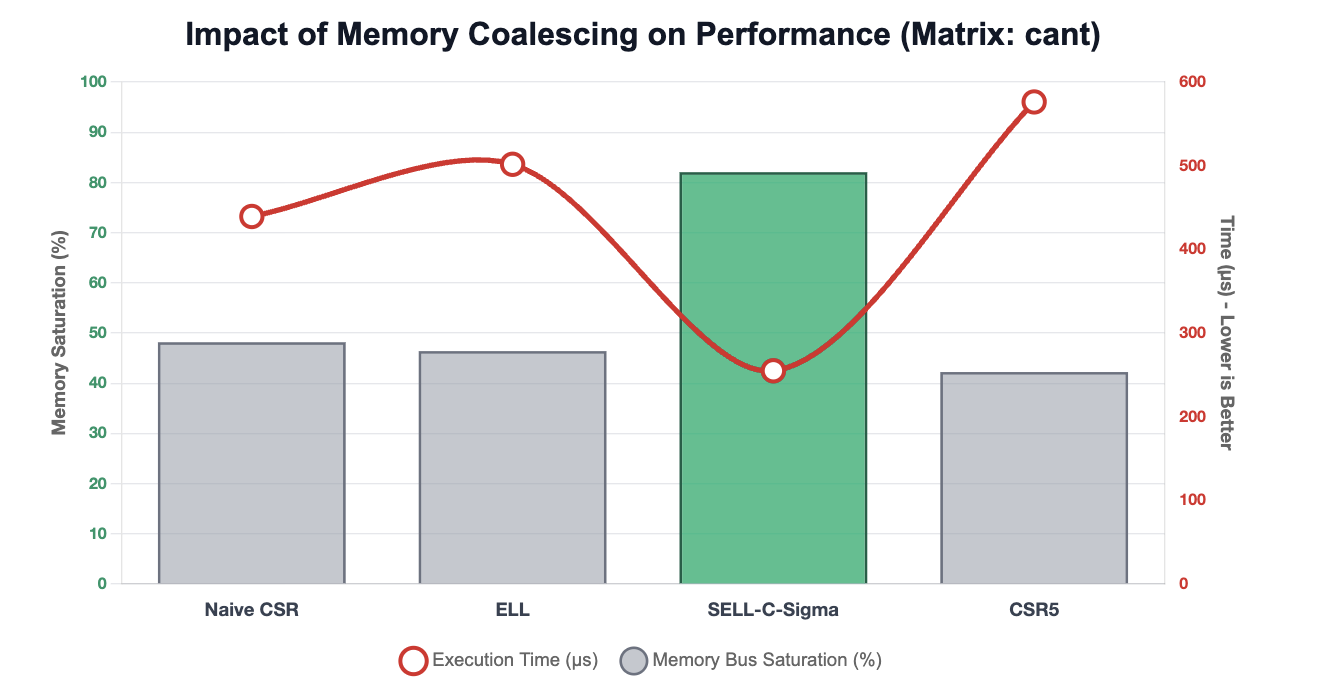
\includegraphics[width=1\linewidth]{mem_coal_performance.png}
    \caption{Impact of Memory Coalescence on SpMV Times on Talapas}
\end{figure*}

\begin{figure*}[p] 
    \centering
    \begin{subfigure}{\linewidth}
        \centering
        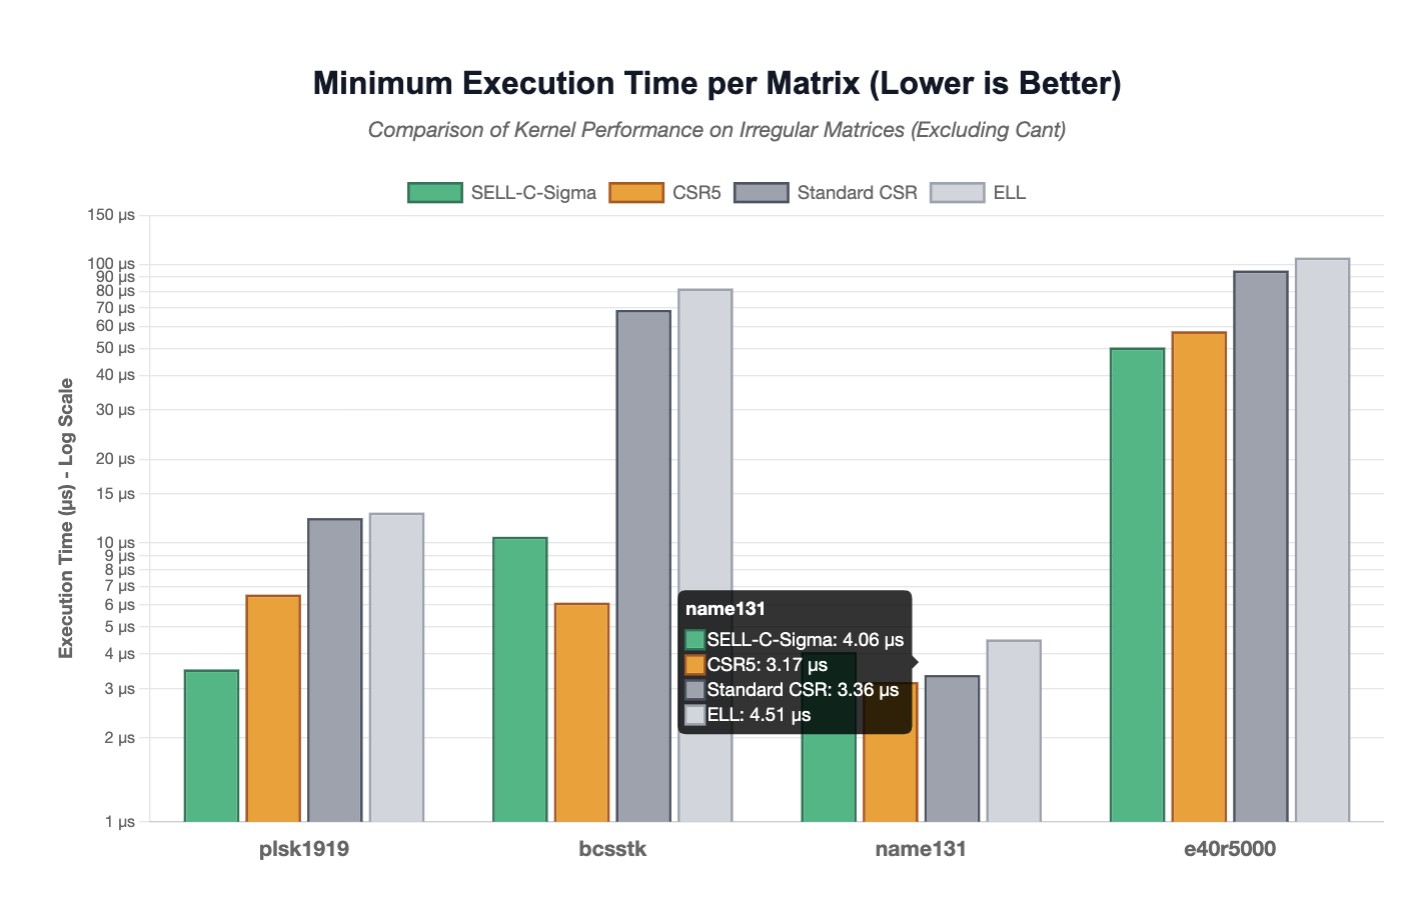
\includegraphics[width=0.8\linewidth]{min_exc_per_mtx.png}
        \caption{Minimum Execution on Talapas}
        \label{fig:placeholder}
    \end{subfigure}
    \vspace{0.2in}
    \begin{subfigure}{\linewidth}
        \centering
        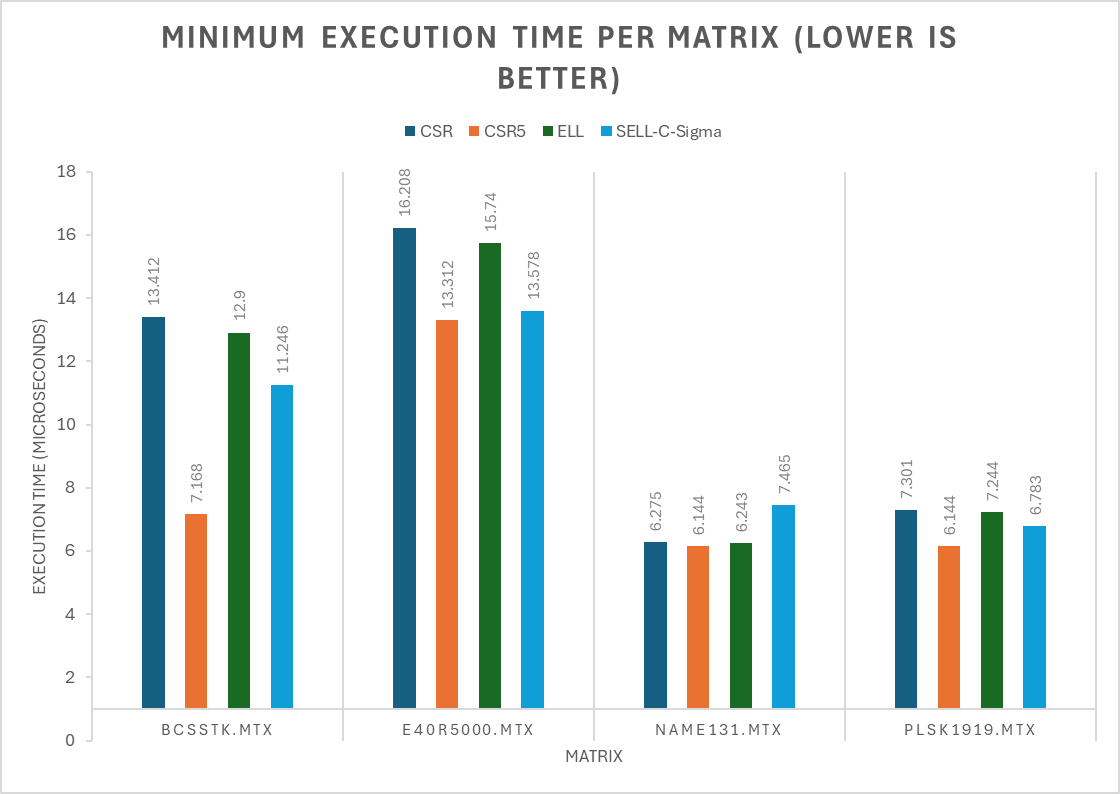
\includegraphics[width=0.8\linewidth]{min_exc_orca.png}
        \caption{Minimum Execution on ORCA}
        \label{fig:placeholder}
    \end{subfigure}
    \caption{Execution Times on Talapas and ORCA} 
\end{figure*}


\begin{figure*}[p]
    \centering
    \begin{subfigure}{\linewidth}
        \centering
        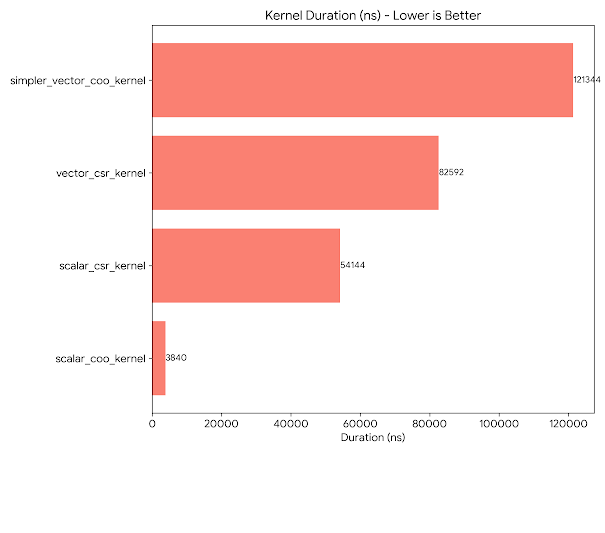
\includegraphics[width=0.5\linewidth]{coo_csr_duration.png}
        \caption{Duration of COO and CSR Kernels}
        \label{fig:image}
    \end{subfigure}
    \begin{subfigure}{\linewidth}
        \centering
        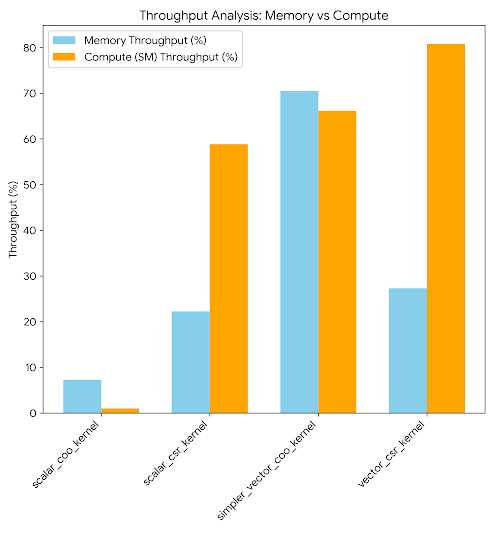
\includegraphics[width=0.5\linewidth]{coo_csr_throughput.png}
        \caption{Memory throughput of COO and CSR Kernels}
        \label{fig:image}
    \end{subfigure}
    \caption{Duration and memory throughput of COO and CSR Kernels}
\end{figure*}

\begin{figure*}[p]
    \centering
    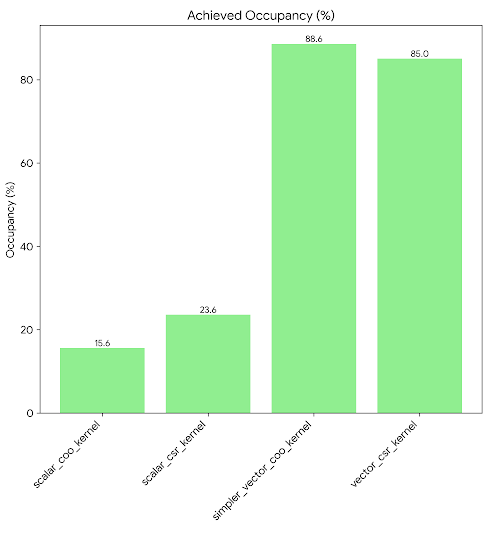
\includegraphics[width=0.5\linewidth]{imgs/coo_csr_occupancy.png}
    \caption{Maximum Occupancy achieved by COO and CSR Kernels}
    \label{fig:image}
\end{figure*}


\begin{thebibliography}{100}


\bibitem{SELLCSIGMA}
Anzt, H., Tomov, S., \& Dongarra, J. (2014, November). 
Implementing a Sparse Matrix Vector Product for the SELL-C/SELL-C-σ formats on NVIDIA GPUs. 
\emph{In 2014 IEEE International Conference on Cluster Computing (CLUSTER)} (pp. 61–66).
\url{https://library.eecs.utk.edu/files/ut-eecs-14-727.pdf}


\bibitem{Bell2008}
Bell, N. \& Garland, M. (2008). Efficient Sparse Matrix-Vector Multiplication on CUDA.
\emph{Nvidia Technical Report NVR-2008-004} Vol. 2. No. 5.

\bibitem{Benatia2018BestSF} Benatia, A., Ji, W., Wang, Y., \& Shi, F. (2018). BestSF: A Sparse Meta-Format for Optimizing SpMV on GPU. \emph{ACM Transactions on Architecture and Code Optimization}, 15(3), 29. \url{https://doi.org/10.1145/3226228}

\bibitem{Flegar2017}
Flegar, G., \& Anzt, H. (2017). Overcoming Load Imbalance for Irregular Sparse Matrices. 
\emph{In Proceedings of the International Conference on Supercomputing (ICS)}, Chicago, IL, USA.
\url{https://publikationen.bibliothek.kit.edu/1000079215}

\bibitem{Gao2016SpMV}
Gao, J., Wang, Y., \& Wang, J. (2016). A novel multi–graphics processing unit parallel optimization framework for the sparse matrix-vector multiplication.
\emph{Concurrency and Computation: Practice and Experience}, 29(17), e3936.
\url{https://doi.org/10.1002/cpe.3936}

\bibitem{Kolodziej2019} 
Kolodziej, S. P., Aznaveh, M., Bullock, M., David, J., Davis, T. A., Henderson, M., Hu, Y. \& Sandstrom, R. (2019). The {SuiteSparse} Matrix Collection Website Interface. \emph{Journal of Open Source Software} Vol. 4. No. 35. pages 1244.

\bibitem{Li2015SpMV}
Li, K., Yang, W., \& Li, K. (2015). Performance Analysis and Optimization for SpMV on GPU Using Probabilistic Modeling. 
\emph{IEEE Transactions on Parallel and Distributed Systems}, 26(1), 196-205.
\url{https://doi.org/10.1109/TPDS.2014.2308221}


\bibitem{Liu2015CSR5}
Liu, W., Vinter, B. (2015). CSR5: An Efficient Storage Format for Cross-Platform Sparse Matrix-Vector Multiplication.
\emph{arXiv preprint arXiv:1503.05032v2 [cs.MS]}.
\url{https://arxiv.org/pdf/1503.05032v2}

\bibitem{NsightCompute2023}
NVIDIA Corporation. (2023). \emph{Nsight Compute Profiling Guide}.
Retrieved from \url{https://docs.nvidia.com/nsight}


\bibitem{nvidia_a100_specs}
NVIDIA. (2020). \emph{NVIDIA A100 Tensor Core GPU Datasheet}. 
Santa Clara, CA: NVIDIA Corporation. 
\url{https://www.nvidia.com/en-us/data-center/l40s/}


\bibitem{orca_pdx_cluster}
Portland State University Research Computing. (2024). \emph{Orca High Performance Computing Cluster Documentation}. 
Describes compute nodes with 6× L40S GPU nodes (24 total GPUs) and 19× A30 GPU nodes (76 total GPUs), 
each with AMD EPYC 9534 CPUs and 576 GB RAM. Retrieved from \url{https://orca.pdx.edu/about/compute-resources/}

\bibitem{Tsai2021Race}
Tsai, Y. M., Cojean, T., \& Anzt, H. (2021). Sparse Linear Algebra on AMD and NVIDIA GPUs – The Race Is On. 
\emph{In Proceedings of the International Conference on High Performance Computing (ISC)}, Virtual Event.
\url{https://doi.org/10.1007/978-3-030-78713-4_11}


\bibitem{talapas_a100}
University of Oregon Research Computing. (2024). \emph{Talapas GPU-Enabled Compute Nodes}.
Documentation for NVIDIA A100 GPU nodes on the Talapas HPC cluster. Retrieved from 
\url{https://racs.uoregon.edu/services}

\end{thebibliography}{100}


\end{multicols}{2}


\end{document}

